\documentclass[10pt]{article}
\usepackage[utf8]{inputenc}
\usepackage[table]{xcolor}
\usepackage{graphicx}
\usepackage{blindtext}
\usepackage{enumitem}
\usepackage{booktabs}


\title{Data document}

\begin{document}

\section{Gather and Prepare Data}

\begin{tabular}{| c | c | c | c | c |}    \toprule
 \textbf{Task} & \textbf{Task Description} & \textbf{\shortstack{Tools Used \\ and Description}} & \textbf{Challenges} & \textbf{\shortstack{How were \\ challenges fixed }}  &&&  \\\midrule
\rowcolor{red!5} Generate Data   & \shortstack{Artifitial data \\ was generated \\ using courses from\\ the faculty \\ information booklet.} & \shortstack{Python write(),\\ Libre Office \\ Spreadsheets(store \\ generated data), \\ import random.} & \shortstack{Artificial data \\ results in \\ poor model \\ performance,\\ lack of cohesion.}  & \shortstack{ Artificial data is \\ relatively sufficient \\ to test and run \\ our prototype, real \\data is needed \\in later versions.} \\ 
\rowcolor{blue!5} \shortstack{Feature \\ Extraction} & \shortstack{The model only \\ needs course \\ symbols as features \\ and the target \\ being the grade \\ to be predicted} & \shortstack{A python script \\ was implemented \\ to access desired \\ features and pass \\ the features to \\ the Data processor.}  & \shortstack{The code for \\ extracting \\ features \\ was order n\\ which took \\ time to execute.} & \shortstack{The features \\ were extracted \\ manually from \\ a file to a \\ separate file thus \\ the training data \\ was in its own file}\\ 
\rowcolor{green!5} \shortstack{Data \\ Preprocessing} & \shortstack{All the feature \\ variables were \\converted from \\ symbols to \\ numerical variables.} & \shortstack{import Pandas, \\ used the pandas \\ library to replace \\ symbols to \\numerical variables} & \shortstack{The processed \\ data had NULL \\ variables. } & \shortstack{All the NULL \\ variables were \\ replaced with \\ a flag numerical \\ value (-1). } \\\bottomrule
 \hline
\end{tabular}

\section{Training the Model}

\begin{tabular}{| c | c | c | c | c |}    \toprule
 \textbf{Task} & \textbf{Task Description} & \textbf{\shortstack{Tools Used \\ and Description}} & \textbf{Challenges} & \textbf{\shortstack{How were \\ challenges fixed }}  &&&  \\\midrule
 \rowcolor{yellow!5}Decision Algorithm & \shortstack{A Decision Tree \\ algorithm was chosen \\ as the preliminary \\ machine learning \\ technique. This \\ was done to give a \\ provisional method \\ for predicting \\ the recommended \\ courses as well \\ the expected grade \\for each course.} & \shortstack{From the Scikit \\ learn library, \\ the built in \\ Decision algorithm \\was utilized to \\ decide whether \\ a student \\ will get good \\ grades for courses \\ that will soon\\ be recommended,\\ if the grades \\ are indeed good \\ the specific \\ courses will be \\ recommended.} & \shortstack{The trained \\ model did \\ not perform \\ in its optimal \\ performance, \\ because the \\ data used\\ to train the \\ model was \\ biased that \\ is , there \\ was no  \\ cohesion \\ amongst \\ features.}  & \shortstack{ Artificial data is \\ relatively sufficient \\ to test and run \\ our prototype, real \\data is needed \\in later versions.} \\ \bottomrule
 \hline
\end{tabular}

\newpage

\section{Detailed description of the dataset}

\subsection{Raw Data}
\begin{description}[font=$\bullet$~\normalfont\scshape\color{red!50!black}]
\item [] The raw data is structured in a .csv file. It consists of 1000 students who did their undergraduate courses.
\item [] The following files : FIRST\_YEAR.csv, SECOND\_YEAR.csv, THIRD\_YEAR.csv, HONOURS.csv and MASTERS.csv  have all the course codes and course descriptions for computer science as stated in the faculty of science information booklet.
\begin{center}
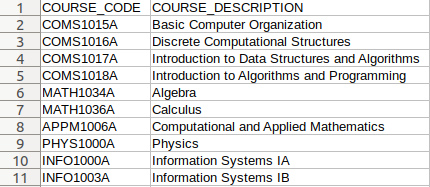
\includegraphics[width=.7\textwidth]{FIRST_YEAR.png}
\end{center}
\caption{Sample of FIRST\_YEAR.csv}

\item[] The STUDENTS.csv contain the details of each user(student).
\begin{center}
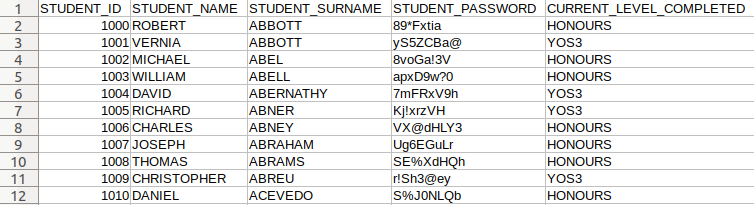
\includegraphics[width=.9\textwidth]{STUDENTS.png}
\end{center}
\caption{Sample of STUDENTS.csv}

\newpage

\item[] The following files : FIRST\_YEAR\_SUB1.csv, SECOND\_YEAR\_SUB1.csv, THIRD\_YEAR\_SUB1.csv, HONOURS\_SUB1.csv contain all the students transcripts. 
\begin{center}
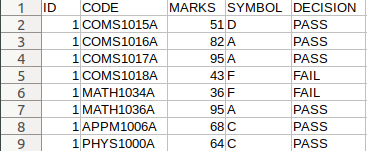
\includegraphics[width=.7\textwidth]{results.png}
\end{center}
\caption{Sample of FIRST\_YEAR\_SUB1.csv showing results for student 1.}
\end{description}

\subsection{Normalized Data}

For the purpose of training our model, the above data needs to be normalized before it is fed into the built-in sklearn Decision Tree Algorithm. Since the 'SYMBOLS' column has been chosen to be the feature for our classifier, we need to convert all the symbols to numerical values. That is, A \rightarrow 0 , B \rightarrow 1 , C \rightarrow 2, D \rightarrow 3, F \rightarrow 4.

If a student did not take part in a particular course, we flag the grade with -1.

\begin{center}
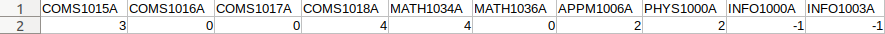
\includegraphics[width=1.0\textwidth]{normalized_features.png}
\end{center}
\caption{Normalized first year results for student 1.}  

\end{document}